\documentclass[10pt, a4paper, italian]{article}
\usepackage[T1]{fontenc}
\usepackage[utf8]{inputenc}
\usepackage{amsmath, amssymb, amsthm, thmtools, amsfonts, mathtools}
\usepackage{nicefrac}
\usepackage{calc}
\usepackage[pdftex, hyperindex, plainpages=false]{hyperref}
\usepackage[nameinlink]{cleveref} %load before classicthesis (clash)
%\usepackage[nochapters,pdfspacing]{classicthesis}
\usepackage{siunitx}
\usepackage[siunitx]{circuitikz}

\usepackage[a4paper]{geometry}
\usepackage{float}
\usepackage{mdframed}
\usepackage{titling}
\usepackage{booktabs}
\usepackage{graphicx}
\usepackage{caption, subcaption}
\usepackage{xcolor}
\usepackage[italian]{babel}
\usepackage{pgfplots}
\usepackage{listings}
%\usepackage{lmodern}
\usepackage{url}
\usepackage{enumitem}
\usepackage{tikz} %loads after classicthesis (xcolor incompat)

% lets graphicx know path where figures to be included are found
\graphicspath{{../figs/}}
\makeatletter
\def\input@path{{../figs/}}
%or: \def\input@path{{/path/to/folder/}{/path/to/other/folder/}}
\makeatother

% tikz pgf plots setup
\usepgfplotslibrary{external}
\pgfplotsset{compat=1.15}
%\tikzexternalize

% spaces and significant digits/figures for measurements
\sisetup{free-standing-units, space-before-unit, number-unit-product = \;,
scientific-notation = false, round-mode = figures, round-precision = 1,}

% turns all (hyperlinked) references black [default is blue]
\hypersetup{
	linktoc=all,
	colorlinks=true,
	linkcolor=black
}

% code listings config
%\lstset{
%language=Python,
%basicstyle=\ttfamily,
%columns=fullflexible,
%keepspaces=true,
%}

% mdframed (for boxed text) configuration
\mdfsetup{linewidth=0.6pt}

% Default fixed font does not support bold face
\DeclareFixedFont{\ttb}{T1}{txtt}{bx}{n}{12} % for bold
\DeclareFixedFont{\ttm}{T1}{txtt}{m}{n}{12}  % for normal

% Custom colors
\usepackage{color}
\definecolor{deepblue}{rgb}{0,0,0.5}
\definecolor{deepred}{rgb}{0.6,0,0}
\definecolor{deepgreen}{rgb}{0,0.5,0}

% Commands 
\newcommand{\executeiffilenewer}[3]{%
	\ifnum\pdfstrcmp{\pdffilemoddate{#1}}%
		{\pdffilemoddate{#2}}>0%
	{\immediate\write18{#3}}\fi%
}
% input .svg --> .pdf_tex graphs
%\newcommand{\includesvg}[1]{%
%	\executeiffilenewer{#1.svg}{#1.pdf}%
%	{inkscape -z -D --file=#1.svg %
%	--export-pdf=#1.pdf --export-latex}%
%	\input{#1.pdf_tex}%
%}
% Thanks UniPi's Department of Physics E. Fermi
\newcommand{\thanksdf}{(\thanks{Dipartimento di Fisica E.~Fermi,%
Universit\`a di Pisa - Pisa, Italy.}\;)}

% hyperlink to email address
\newcommand{\mail}[1]{\href{mailto:#1}{\textsf{#1}}}

% \vec for bold vectors, instead of overarrows (now "\arrvec")
\let\arrvec=\vec
\renewcommand{\vec}[1]{\boldsymbol #1}
% replaces straight phi with slanted phi
\renewcommand{\phi}{\varphi}
% replaces straight eps with curved epsilon
\newcommand{\eps}{\varepsilon}
% abbreviation for (sub_/super^)scripts of \lim, \sum,... in inline math
\newcommand{\ds}{\displaystyle}

% blackboard/number set letters
\newcommand{\CC}{\mathbb C}
\newcommand{\HH}{\mathbb H}
\newcommand{\KK}{\mathbb K}
\newcommand{\NN}{\mathbb N}
\newcommand{\PP}{\mathbb P}
\newcommand{\QQ}{\mathbb Q}
\newcommand{\RR}{\mathbb R}
\newcommand{\ZZ}{\mathbb Z}

\newcommand{\Abs}[1]{{\left\Vert #1\right\Vert}}
\newcommand{\enclose}[1]{{\left( #1 \right)}}
\newcommand{\Enclose}[1]{{\left[ #1 \right]}}
\newcommand{\floor}[1]{\left\lfloor #1 \right\rfloor}
\newcommand{\ceil}[1]{\left\lceil #1 \right\rceil}
\newcommand{\To}{\rightrightarrows}

% Math operators
\DeclareMathOperator{\divergence}{div}
\renewcommand{\div}{\divergence}
\DeclareMathOperator{\Imaginarypart}{Im}
\renewcommand{\Im}{\Imaginarypart}
\DeclareMathOperator{\Realpart}{Re}
\renewcommand{\Re}{\Realpart}
%\DeclareMathOperator{\arg}{arg}
\DeclareMathOperator{\tg}{tg}
\DeclareMathOperator{\arctg}{arctg}
\DeclareMathOperator{\settsinh}{settsinh}
\DeclareMathOperator{\settcosh}{settcosh}
\DeclareMathOperator{\tr}{tr}
\DeclareMathOperator{\im}{im}
\DeclareMathOperator{\sgn}{sgn}
\DeclareMathOperator{\diag}{diag}

\DeclarePairedDelimiter{\norm}{\lVert}{\rVert}
\DeclarePairedDelimiter{\scalar}{\langle}{\rangle}

% Logarithm with arbitrary base.
% -> log_10
\newcommand{\llog}[1][10]{\log_{#1}}

% Absolute value.
% -> |x|
\newcommand{\abs}[1]{\left| #1 \right|}

% Powers.
% -> x^a
\newcommand{\power}[2][2]{\left( #2 \right)^{#1}}

% Square.
% -> x^2
\newcommand{\sq}[1]{\power[2]{#1}}

% Expansion of the binomial coefficient.
% -> n1!/(n2!(n1 - n2)!)
\newcommand{\binomexpr}[2]{\frac{#1!}{#2!(#1 - #2)!}}

% Expression evaluation at a given point with square brackets.
% -> [x]_{a}
\newcommand{\at}[2]{\left[ #1\right]_{\makebox[-1pt][l]{${\scriptstyle#2}$}}}

% Expression evaluation in an interval.
% -> [x] _{a}^{b}
\newcommand{\eval}[3]{\left.#1%
  \right|_{\makebox[-1pt][l]{${\scriptstyle#2}$}}^{\makebox[-1pt][l]{${\scriptstyle#3}$}}}

% Upright d in math mode (for differentials).
% -> d
\newcommand{\ud}{\mathrm{d}}

% Differential.
% -> dx
\newcommand{\diff}[1][x]{\,\ud{#1}}

% Base command for defining derivatives.
% -> df/dx or d^kf/dx^k
\newcommand{\basederivative}[4][]{%
  \displaystyle%
  \ifx\\#1\\\frac{#4#2}{#4#3}%
  \else%
  \frac{#4^#1#2}{#4#3^#1}%
  \fi%
}

% Total derivative.
% -> df/dx(x) or d^kf/dx^k(x)
\newcommand{\td}[4][]{%
  \basederivative[#1]{#2}{#3}{\ud}%
  \ifx\\#4\\%
  \else%
  \mkern-4mu\left(#4\right)%
  \fi%
}

% Partial derivative.
% -> df/dx(x) or d^kf/dx^k(x)
\newcommand{\pd}[4][]{%
  \basederivative[#1]{#2}{#3}{\partial}%
  \ifx\\#4\\%
  \else%
  \mkern-4mu\left(#4\right)%
  \fi%
}

\newcommand{\intinf}{\int_{-\infty}^{\infty}\!\!\!}

\newcommand{\cinterval}[2]{\left[\, #1,~#2 \,\right]}

\newcommand{\linterval}[2]{\left[\, #1,~#2 \,\right)}

\newcommand{\rinterval}[2]{\left(\, #1,~#2 \,\right]}

\newcommand{\ointerval}[2]{\left(\, #1,~#2 \,\right)}

\newcommand{\prob}[1]{\displaystyle P\left(#1\right)}

\newcommand{\pvalue}{\emph{$p$-value}}

\newcommand{\cond}{\,|\,}

\newcommand{\expect}[1]{\displaystyle E\left[#1\right]}

\newcommand{\mom}[2][]{\displaystyle {\cal M}_{#2}\ifx\\#1\\\else(#1)\fi}

\newcommand{\momalg}[1]{\displaystyle \lambda_{#1}}

\newcommand{\momcen}[1]{\displaystyle \mu_{#1}}

\newcommand{\skewness}{\displaystyle \gamma_1}

\newcommand{\kurtosis}{\displaystyle \gamma_2}

\newcommand{\charf}[1][x]{\phi_{#1}}

\newcommand{\momgenf}[1][x]{M_{#1}}

\newcommand{\fwhm}{{\scriptstyle \textsc{FWHM}}}

\newcommand{\hwhm}{{\scriptstyle \textsc{HWHM}}}

\newcommand{\median}{\mu_{\nicefrac{1}{2}}}

\newcommand{\var}[1]{\ensuremath{\text{Var}\left(#1\right)}}

\newcommand{\cov}[2]{\ensuremath{\text{Cov}\left(#1, #2\right)}}

\newcommand{\corr}[2]{\ensuremath{\text{Corr}\left(#1, #2\right)}}

\newcommand{\like}{\mathcal L}

\newcommand{\likelihood}[2][]{\like\ifx\\#2\\\else(#2\ifx\\#1\\\else;#1\fi)\fi}

\newcommand{\chisq}{\ensuremath{\chi^2}}

\newcommand{\chisquare}[2][]{\chisq\ifx\\#2\\\else(#2\ifx\\#1\\\else;#1\fi)\fi}

\newcommand{\loglikelihood}[2][]{\log\likelihood[#1]{#2}}

\newcommand{\pdf}[3][]{#2(#3\ifx\\#1\\\else;#1\fi)}

\newcommand{\binomialpdf}[2][]{\pdf[#1]{\mathcal B}{#2}}

\newcommand{\multinomialpdf}[2][]{\pdf[#1]{\mathcal M}{#2}}

\newcommand{\poissonpdf}[2][]{\pdf[#1]{\mathcal P}{#2}}

\newcommand{\uniformpdf}[2][]{\pdf[#1]{u}{#2}}

\newcommand{\exponentialpdf}[2][]{\pdf[#1]{\varepsilon}{#2}}

\newcommand{\gausspdf}[2][]{\pdf[#1]{N}{#2}}

\newcommand{\chisquarepdf}[2][]{\pdf[#1]{\wp}{#2}}

\newcommand{\cauchypdf}[2][]{\pdf[#1]{c}{#2}}

\newcommand{\erf}[1]{\ensuremath{\text{erf}\left(#1\right)}}

\newcommand{\dccases}[4][]{#2 \ifx\\#2\\\else=\fi %
  \begin{cases}
    \displaystyle #3 & \text{per variabili discrete}\\
    \displaystyle #4 & \text{per variabili continue}#1
  \end{cases}
}
% sub/super-scriptable for all symbol as math operator 
\newcommand\Scaleforall[1]{\vcenter{\hbox{\scalefont{#1}$\forall$}}}

\DeclareMathOperator*\forevery{%
  \vphantom\sum
  \mathchoice{\Scaleforall{2}}{\Scaleforall{1.4}}{\Scaleforall{1}}{\Scaleforall{0.75}}}
\geometry{left=2cm, right=2cm, top=2cm, bottom=2cm}

% indexes subsections with letters, sections with numbers (1.a, 1.b, ...)
\renewcommand{\thesubsection}{\thesection.\alph{subsection}}

% lets graphicx know path where figures to be included are found
\graphicspath{{../figs/}}

\author{Gruppo 1.AC \\ Matteo Rossi}
\title{Es06A: Oscillatore sinusoidale a ponte di Wien con Amplificatore Operazionale}
\begin{document}
\date{\today}
\maketitle

\setcounter{section}{0}

\section*{Misura componenti dei circuiti}
\begin{table}[htbp]
\centering
\begin{tabular}{cccccc}
\toprule
Resistenze $[\si{k\ohm}]$ & $R$ & $\sigma R$ & Capacità $[\si{n\F}]$ & $C$ &
$\sigma C$ \\
\midrule
\midrule
$R_1$	  & 9.96 	& 0.8 	 & $C_2$ & 10.5		 & 0.4 \\
$R_2$	  & 9.95	& 0.08 	 & $C_1$ & 9.6		 & 0.4 \\
$R_3$	  & 9.97	& 0.08	 & & & \\
$R_4$	  & 9.97	& 0.08	 & & & \\
$R_5$	  & 9.93	& 0.08	 & & & \\
\bottomrule     
\end{tabular}
\caption{Valori di resistenza e capacità misurate per i componenti dei
circuiti studiati. \label{tab: rcmes}}
\end{table}

\subsection*{Nota sul metodo di fit}
Per determinare i parametri ottimali e le rispettive covarianze si \`e
implementato in \verb+Python+ un algoritmo di fit basato sui minimi quadrati
mediante la funzione \emph{curve\_fit} della libreria \texttt{SciPy}.

%=======================
\section{Misura del loop-gain $\beta A_v$}
Dopo aver preparato i componenti ed averli correttamente misurati,s i è montato il circuito per la misura del loop-gain
$\beta(j\omega) \bar{A}$ tramite il circuito nello schema in \cref{fig: Draft1}
\begin{figure}[H]
    \centering
	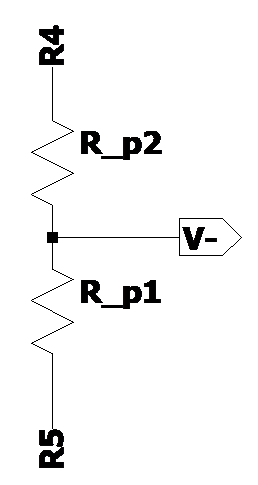
\includegraphics[scale=0.5]{Draft3}
    \caption{Schema circuitale di massima per il funzionamento del potenziometro $POT_1$.
    \label{fig: Draft3}}
\end{figure}
\begin{figure}[H]
    \centering
	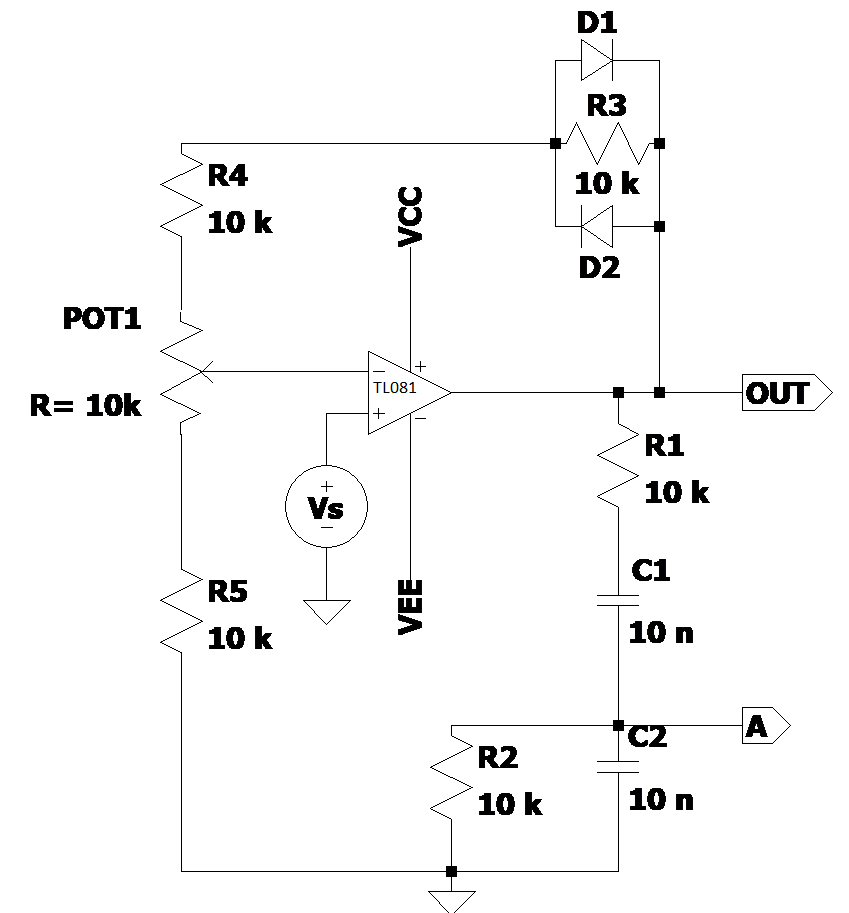
\includegraphics[scale=0.5]{Draft1}
    \caption{Schema circuitale per misurare il loop-gain.
    \label{fig: Draft1}}
\end{figure}

Il circuito è formato da due sottocircuiti collegati in serie: il primo è un amplificatore non invertente formato dall'opAmp,$R_3$,$R_4$,$POT_1$ (che a sua volta può essere considerato come la somma di due resistenze in serie $R_{p1}$ e $R_{p2}$, posizionati come in \cref{fig: Draft3}) e $R_5$; si è trascurato l'effetto dei diodi dal momento in cui $V_{R_3}$ sarà sempre molto inferiore al $V_\gamma$ dei diodi $\approx 0.7 \si{V}$, non permettendogli di andare in conduzione.
Il guadagno di questo anello è quindi governato dalla legge 
\begin{equation}\label{eq: AinPot}
A  = 1 + \frac{R_{p2} + R_3 + R_4}{R_{p1} + R_5}
\end{equation}
Per completezza si è misurato anche la resistenza totale del potenziometro $R_{POT}=9.84 \pm 0.08 \si{k\ohm}$.
Il secondo sottocircuito invece è una rete di feedback positivo costruito con due impedenze, una in serie e l'altra in parallelo
\begin{equation}\label{eq: A}
Z_S (R_1,C_1) = R_1 + \frac{1}{s C_1} = R_1 \frac{s + \frac{1}{C_1 R_1}}{s} \\
\end{equation}
\begin{equation}\label{eq: B}
Z_P (R_2,C_2) = \frac{R_2}{1 + s R_2 C_2} = R_2 \frac{\frac{1}{C_2 R_2}}{s + \frac{1}{C_2 R_2}}
\end{equation}
che definiscono un guadagno pari a
\begin{equation} \label{eq:loop-gain-beta}
\beta = \frac{Z_P}{Z_S + Z_P} = \frac{1}{Z_S/Z_P + 1}
\end{equation}
Chiamando $\omega_1 = 1/(R_1 C_1)$ e $\omega_2 = 1/(R_2 C_2)$ e sviluppando l'equazione, si ottiene
\begin{equation}
\beta(s) = \frac{1}{1 + Z_S/Z_P} =
\frac{1}{1 + \frac{R_1}{R_2} \frac{(s + \omega_1)(s + \omega_2)}{s \omega_2}} =
\frac{R_2}{R_1} \frac{s \omega_2}{\omega_1 \omega_2 + s^2 +
\left[\omega_{1} + \omega_{2} \left(1 + \frac{R_2}{R_{1}}\right)\right] s}
\end{equation}
Per le condizioni di Barkhausen, sostituendo $s = j\omega$
\begin{equation} \label{eq:bark}
\beta(j\omega) = \frac{R_2}{R_1} \frac{j \omega \omega_2}
{\omega_1 \omega_2 - \omega^2 + j \omega
\left[\omega_1 + \omega_2 \left(1 + \frac{R_2}{R_1}\right)\right]} \in \RR^+
\end{equation}
Da cui impongo (per fare in modo che le unità immaginarie si cancellino)
\[
\omega_1 \omega_2 - \omega_0^2 = 0\\
\]
\[
\omega_0 =\sqrt{\omega_1 \omega_2}
\]
Se però vado a sostituire i valori nominali, dato che tutte le resistenze sarebbero uguali tra di loro $= 10 \si{k\ohm}$ e anche le capacità $= 10 \si{\nano\F}$, il guadagno complessivo $L(j\omega)$ diventa
\[
\tilde{\omega}=\frac{1}{RC}\\
\]
\[
\omega_0 =\sqrt{\omega_1 \omega_2} \implies \omega_0=\tilde{\omega}
\]
\[
L(j\tilde{\omega})=A\beta(j\tilde{\omega})=A \frac{\tilde{\omega}}{3\tilde{\omega}}=\frac{A}{3}
\]
Infine, dato che l'oscillazione deve autosostenersi ed essere stabile, c'è bisogno che il guadagno complessivo dei 2 anelli sia $=1$, il che vuol dire che ci sarà bisogno di spostare il potenziometro affinché il guadagno dell'amplificatore invertente diventi $=3$, e inoltre di trovare la frequenza $\omega_0$ per cui il guadagno del loop di feedback sia $=3$
\subsection{Risposta in frequenza e misura di $\omega_0$}
Utilizzando la funzione Network di Waveforms si è pilotato il circuito con un'onda sinusoidale di ampiezza picco-picco di $200 \si{m\V}$, e abbiamo misurato la risposta in frequenza del circuito all'uscita A essendo 
\[
\frac{V_A}{V_s} = \beta(j\omega) \bar{A} = \bar{L}(j\omega)
\]
\begin{figure}[H]
    \centering
	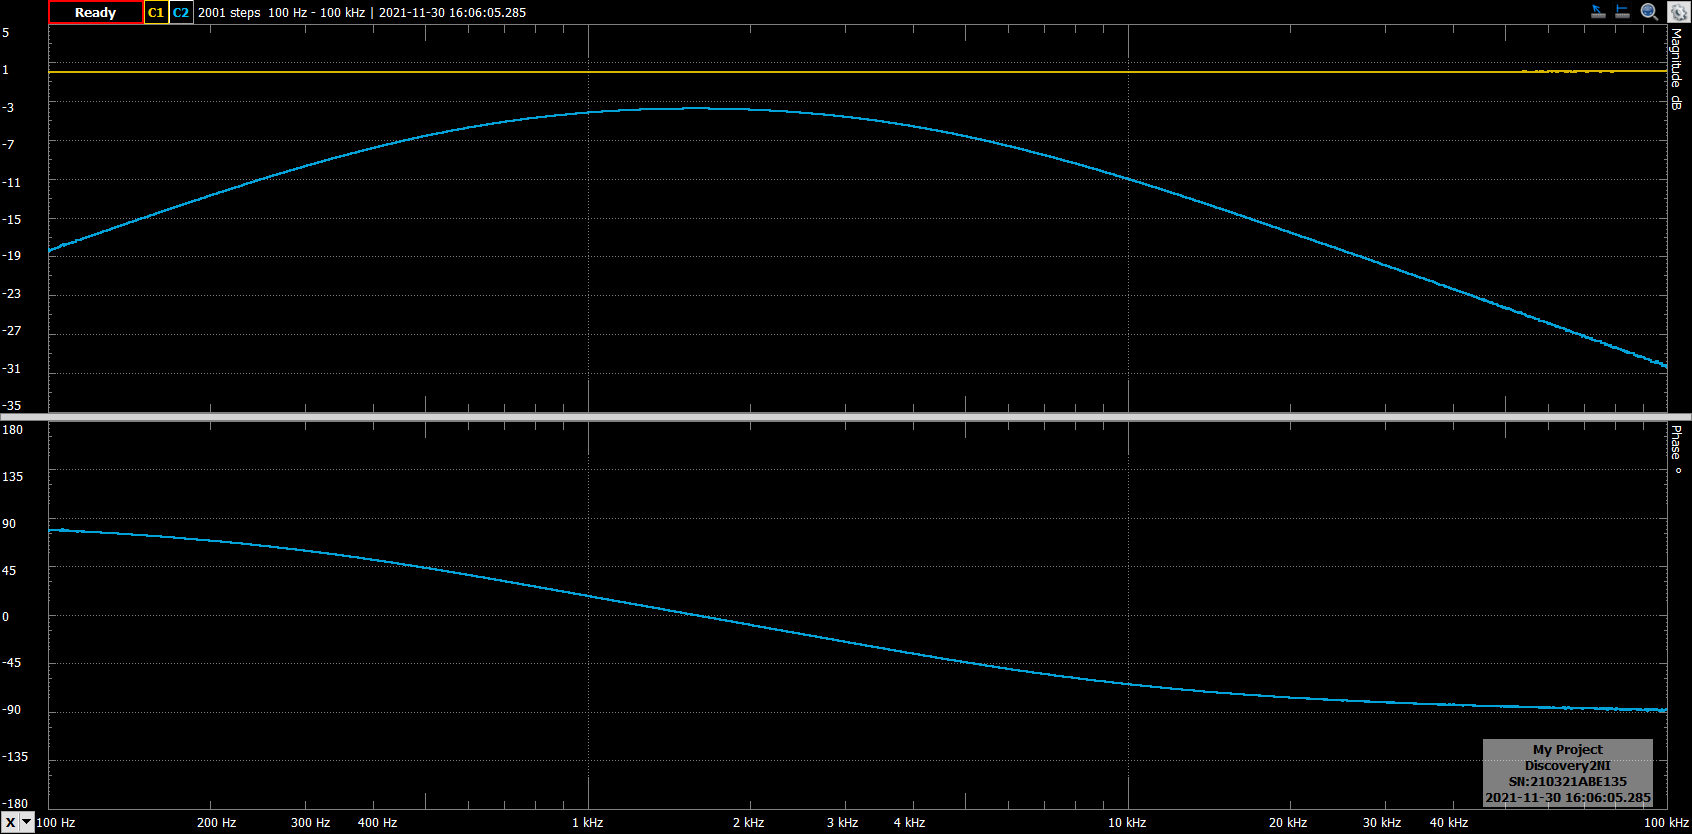
\includegraphics[scale=0.5]{3a}
    \caption{Plot di network tra 100 Hz e 100 kHz del circuito in \cref{fig: Draft1} in risposta ad un'onda sinusoidale di ampiezza picco-picco di 200 mV }
    \label{fig: 3a}
\end{figure}
Utilizzando poi i cursori che fornisce il programma abbiamo misurato la frequenza a cui lo sfasamento si annullava, ed abbiamo ricavato 
\[
f_0=1.58 \pm 0.02 \si{k\Hz}
\]
Teoricamente invece mi aspetto un valore di
\[
f_0 =\frac{\sqrt{\omega_1 \omega_2}}{2\pi}=1.59 \pm 0.05 \si{k\Hz}
\]
Si vede subito che la misura è quindi perfettamente compatibile con quanto ci aspettavamo nella teoria.
Infine abbiamo anche attivato il plot di Nyquist nello stesso modo con cui abbiamo visualizzato la risposta in frequenza.
\begin{figure}[H]
    \centering
	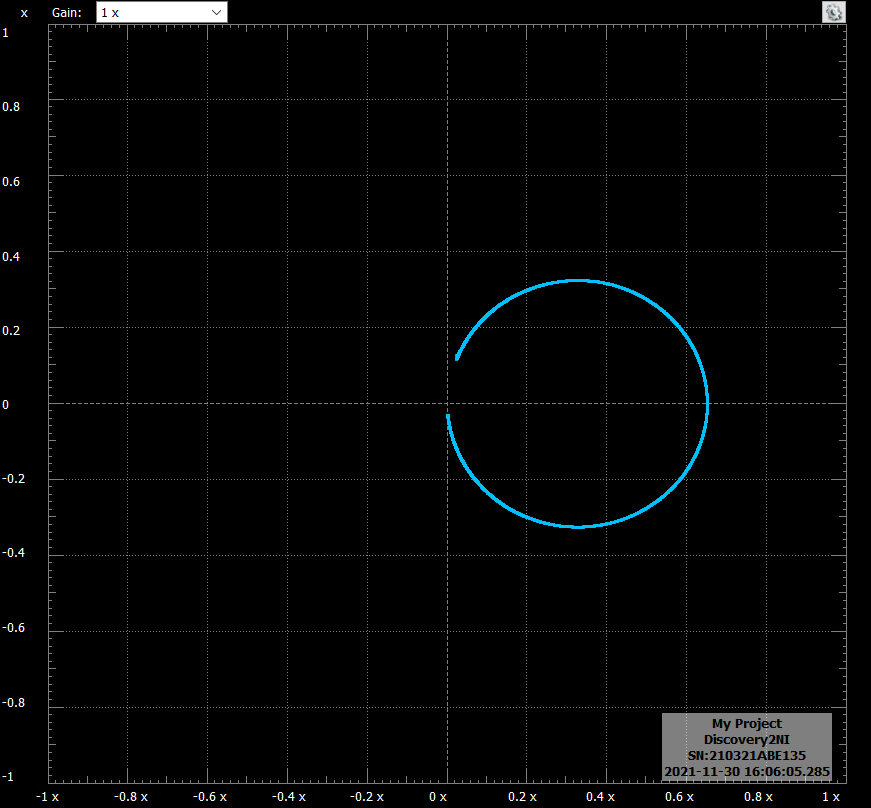
\includegraphics[scale=0.5]{3a_nyquist}
    \caption{Plot di Nyquist tra 100 Hz e 100 kHz del circuito in \cref{fig: Draft1} in risposta ad un'onda sinusoidale di ampiezza picco-picco di 200 mV }
    \label{fig: 3a_nyquist}
\end{figure}
\subsection{Dipendenza dal valore del potenziometro}
Abbiamo misurato come il guadagno cambiasse in funzione della posizione del potenziometro (onde sinusoidali sempre con la stessa frequenza $f_0$ misurata al punto precedente), misurando le resistenza $R_{p1}$, $R_{p2}$, l'ampiezza dell'onda in entrata e in uscita da Out.
\begin{table}[H]
\centering
\begin{tabular}{@{}lllll@{}}
\toprule
$R_{p1} [\si{\ohm}]$  & $R_{p2} [\si{\ohm}]$ & $V_{s} [\si{m\V}]$ & $V_{A} [\si{m\V}]$ & $A_v$ \\
\midrule
$9.32 \pm 0.08 k$ &	$827 \pm 7$	& $201 \pm 2$ 	& $ 409 \pm 4$	& $2.03 \pm 0.03$\\
$8.15 \pm 0.07 k$ &	$1.99 \pm 0.02 k$	& $201 \pm 2$ 	& $ 433 \pm 4$	&$2.15 \pm 0.03$\\
$7.42 \pm 0.06 k$ &	$2.73 \pm 0.03 k$	& $201 \pm 2$ 	&$ 450 \pm 4$	&$2.24 \pm 0.03$\\
$6.98 \pm 0.06 k$ &	$3.17 \pm 0.03 k$	& $201 \pm 2$ 	&	$ 463 \pm 4$&$2.30 \pm 0.03$\\
$4.91 \pm 0.04 k$ &	$5.24 \pm 0.05 k$	& $201 \pm 2$ 	&	$ 527 \pm 5$&$2.62 \pm 0.03$\\
$3.66 \pm 0.04 k$ &	$6.49 \pm 0.06 k$	& $201 \pm 2$ 	&$ 575 \pm 5$	&$2.86 \pm 0.04$\\
$2.70 \pm 0.03 k$ &	$7.45 \pm 0.06 k$	& $201 \pm 2$ 	&$ 619 \pm 5$	&$3.08 \pm 0.04$\\
$1457 \pm 12 $ &	$8.69 \pm 0.07 k$	& $201 \pm 2$ 	&	$ 687 \pm 6$&$3.42 \pm 0.04$\\
$909 \pm 8 $ &	$9.32 \pm 0.08 k$	& $201 \pm 2$ 	&$ 724 \pm 6$	&$3.60 \pm 0.04$\\
$551 \pm 5 $ &	$9.60 \pm 0.08 k$	& $201 \pm 2$ 	&	$ 749 \pm 6$&$3.72 \pm 0.05$\\

\bottomrule
\end{tabular}
\caption{Misura del guadagno in funzione della posizione del potenziometro}
\end{table}
Chiaramente si vede subito che come ci si aspettava dall'equazione (1) di A in funzione delle varie resistenze, cambiando il valore del potenziometro il guadagno non cambia linearmente: per verificare quanto detto si è condotto un fit basato sui minimi quadrati con python sulla stessa equazione, sostituendo $R_{p1} = p R_{pot}$ e $R_{p2}=(1-p)R_{pot}$ e utilizzando $p \in [0,1]$ come variabile, e $R_{pot}$ come incognita.
\begin{figure}[H]
    \centering
	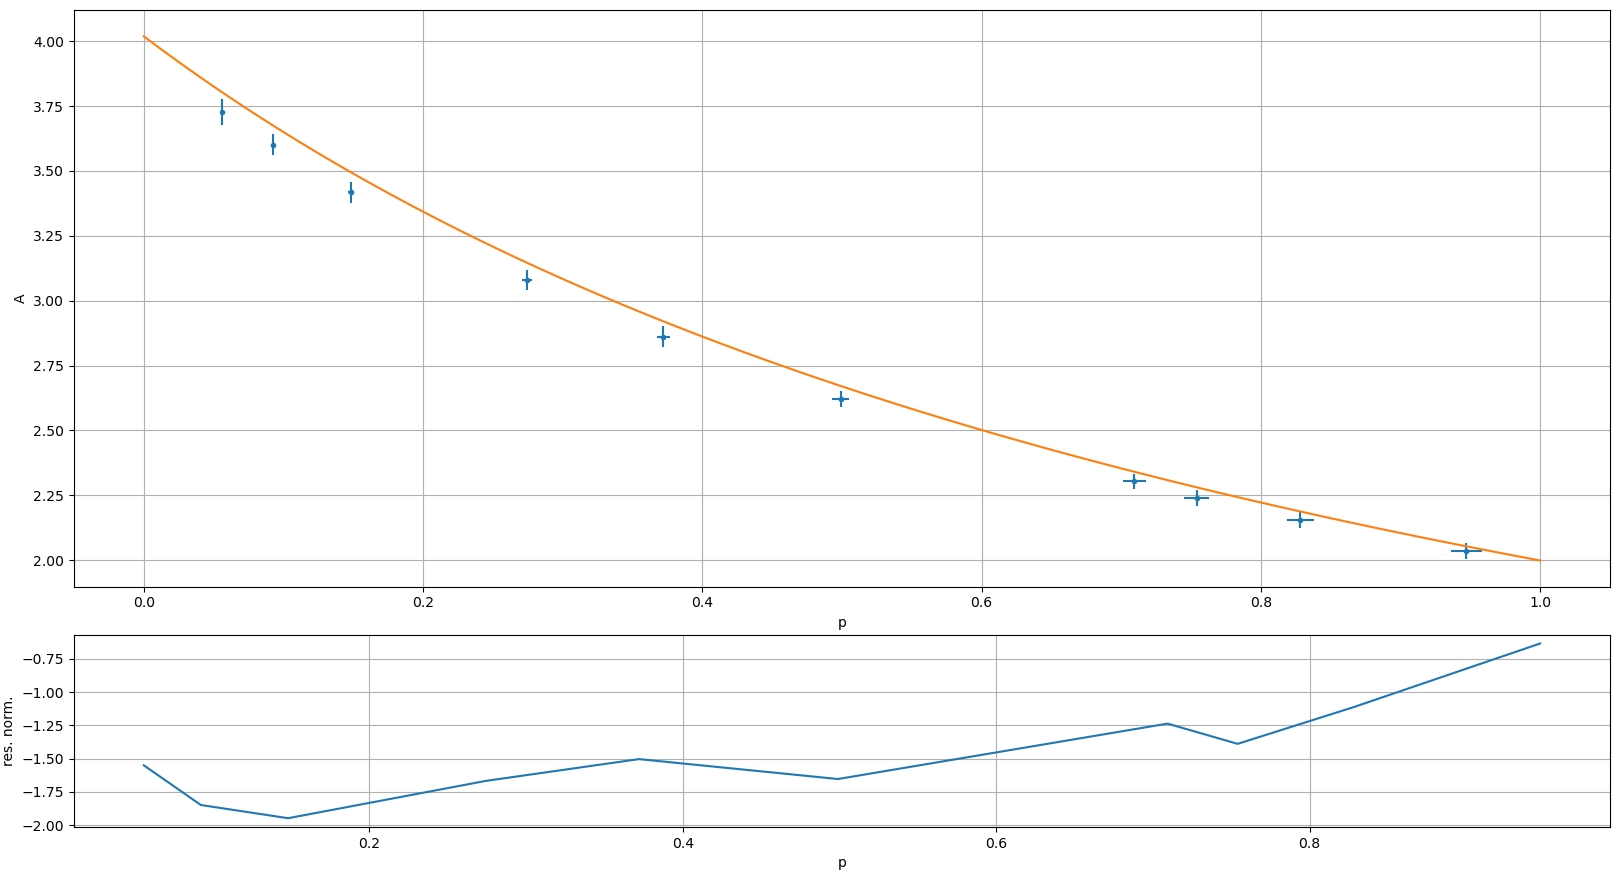
\includegraphics[scale=0.4]{arinzarunza}
    \caption{Fit dell'equazione (1)
    \label{fig: Draft1}}
\end{figure}
Di seguito i valori che si sono riscontrati:\\
$R_{pot}=10.0 \pm 0.4 \si{k\ohm}$\\$chisq=23.1$\\$ndof=9$\\
Da questo si deduce che il modello è compatibile con le misure entro la prima barra di errore.
\subsection{Dipendenza dall'ampiezza dell'onda in ingresso}
Come nella sezione precedente si è inviato al circuito un'onda di ampiezza variabile e frequenza fissata a $f_0$, misurando di volta in volta l'ampiezza dell'onda in entrata e uscita da Out calcolandone il guadagno. Durante le misure si è tenuta fissata anche la posizione del potenziometro a $R_{p1}=3.28 \pm 0.03 \si{k\ohm}$ e $R_{p2}=6.89 \pm 0.06\si{k\ohm}$
\begin{table}[H]
\centering
\begin{tabular}{@{}lllll@{}}
\toprule
$V_{s} [\si{m\V}]$ & $V_{A} [\si{\V}]$ & $A_v$ \\
\midrule
$201 \pm 2$ 	& $ 593 \pm 5 m$	& $2.95 \pm 0.04$\\
$301 \pm 3$ 	& $ 888 \pm 7 m$	& $2.95 \pm 0.04$\\
$401 \pm 4$ 	& $ 1181 \pm 11 m$	& $2.95 \pm 0.04$\\
$501 \pm 4$ 	& $ 1478 \pm 13 m$	& $2.95 \pm 0.04$\\
$601 \pm 6$ 	& $ 1773 \pm 15 m$	& $2.95 \pm 0.04$\\
$702 \pm 6$ 	& $ 2.06 \pm 0.02$	& $2.94 \pm 0.04$\\
$802 \pm 7$ 	& $ 2.35 \pm 0.02$	& $2.93 \pm 0.04$\\
$902 \pm 8$ 	& $ 2.37 \pm 0.02$	& $2.92 \pm 0.04$\\
$1002 \pm 9$ 	& $ 2.90 \pm 0.03$	& $2.90 \pm 0.04$\\
$1103 \pm 10$ 	& $ 3.19 \pm 0.03$	& $2.88 \pm 0.04$\\


\bottomrule
\end{tabular}
\caption{Misura del guadagno in funzione dell'ampiezza dell'onda in ingresso con frequenza e posizione del potenziometro fissati}
\end{table}
Da questi dati ne deduciamo subito che il guadagno tende a diminuire con l'aumentare dell'ampiezza dell'onda in ingresso. Questo perchè finchè il valore di $V_{out}$ permette a $V_{R_3}$ di essere inferiore alla tensione di soglia del diodo, l'amplificazione è lineare e costante (perchè in questo caso i diodi, non essendo polarizzati direttamente, hanno una resistenza tale che il nodo possa esser schematizzato circa con solo la presenza di $R_3$), quando però $V_{out}$ aumenta, aumenterà di conseguenza $V_{R_3}$, i diodi entreranno in polarizzazione diretta, la resistenza del diodo diminuisce insieme alla resistenza del nodo, e quindi diminuirà anche il guadagno dell'anello. L'uscita dell'opAmp resta quindi confinata nell'intervallo di linearità.

%=======================
\section{Oscillatore}
Connettendo il punto A con l'entrata non invertente dell'opAmp si è costruito l'oscillatore a ponte di Wien, come schematizzato in figura \cref{fig: Draft2}
\begin{figure}[H]
    \centering
	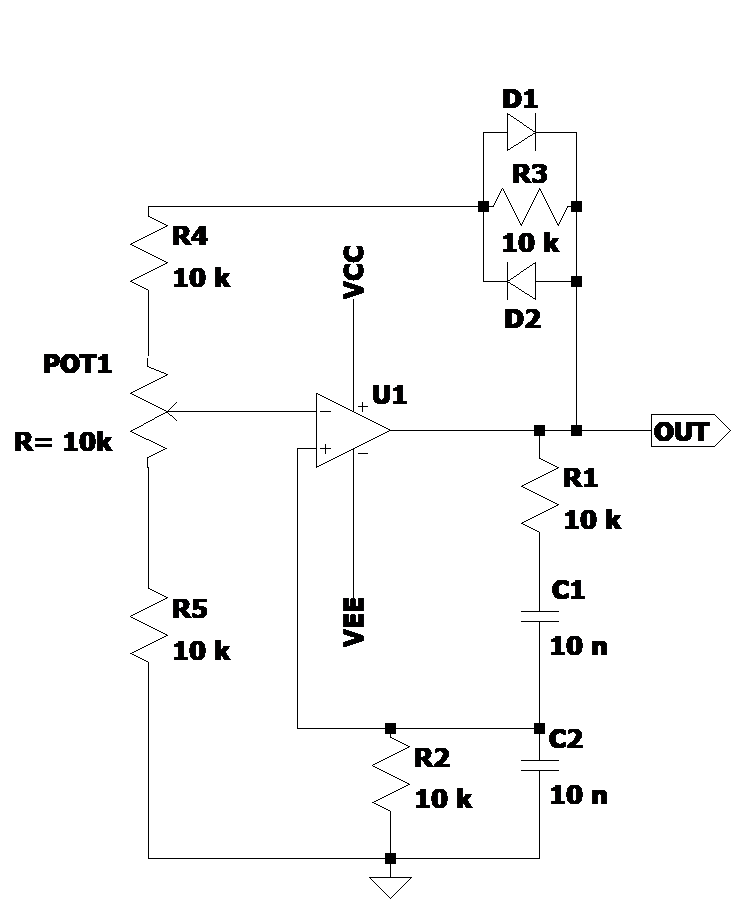
\includegraphics[scale=0.5]{Draft2}
    \caption{Schema circuitale dell'oscillatore a ponte di Wien.
    \label{fig: Draft2}}
\end{figure}
\subsection{Dipendenza dal valore del potenziometro}
Cambiando il valore del potenziometro cambia la forma della'onda in $V_{out}$: quando il valore di $R_{p2}$ è troppo elevato il guadagno dell'anello amplificatore tende a divergere fino alla saturazione; in questa condizione qualunque segnale stabile (anche nullo) finirebbe col divergere, infatti questo comportamento è quello che utilizzeremo come innesco.
\begin{figure}[H]
    \centering
	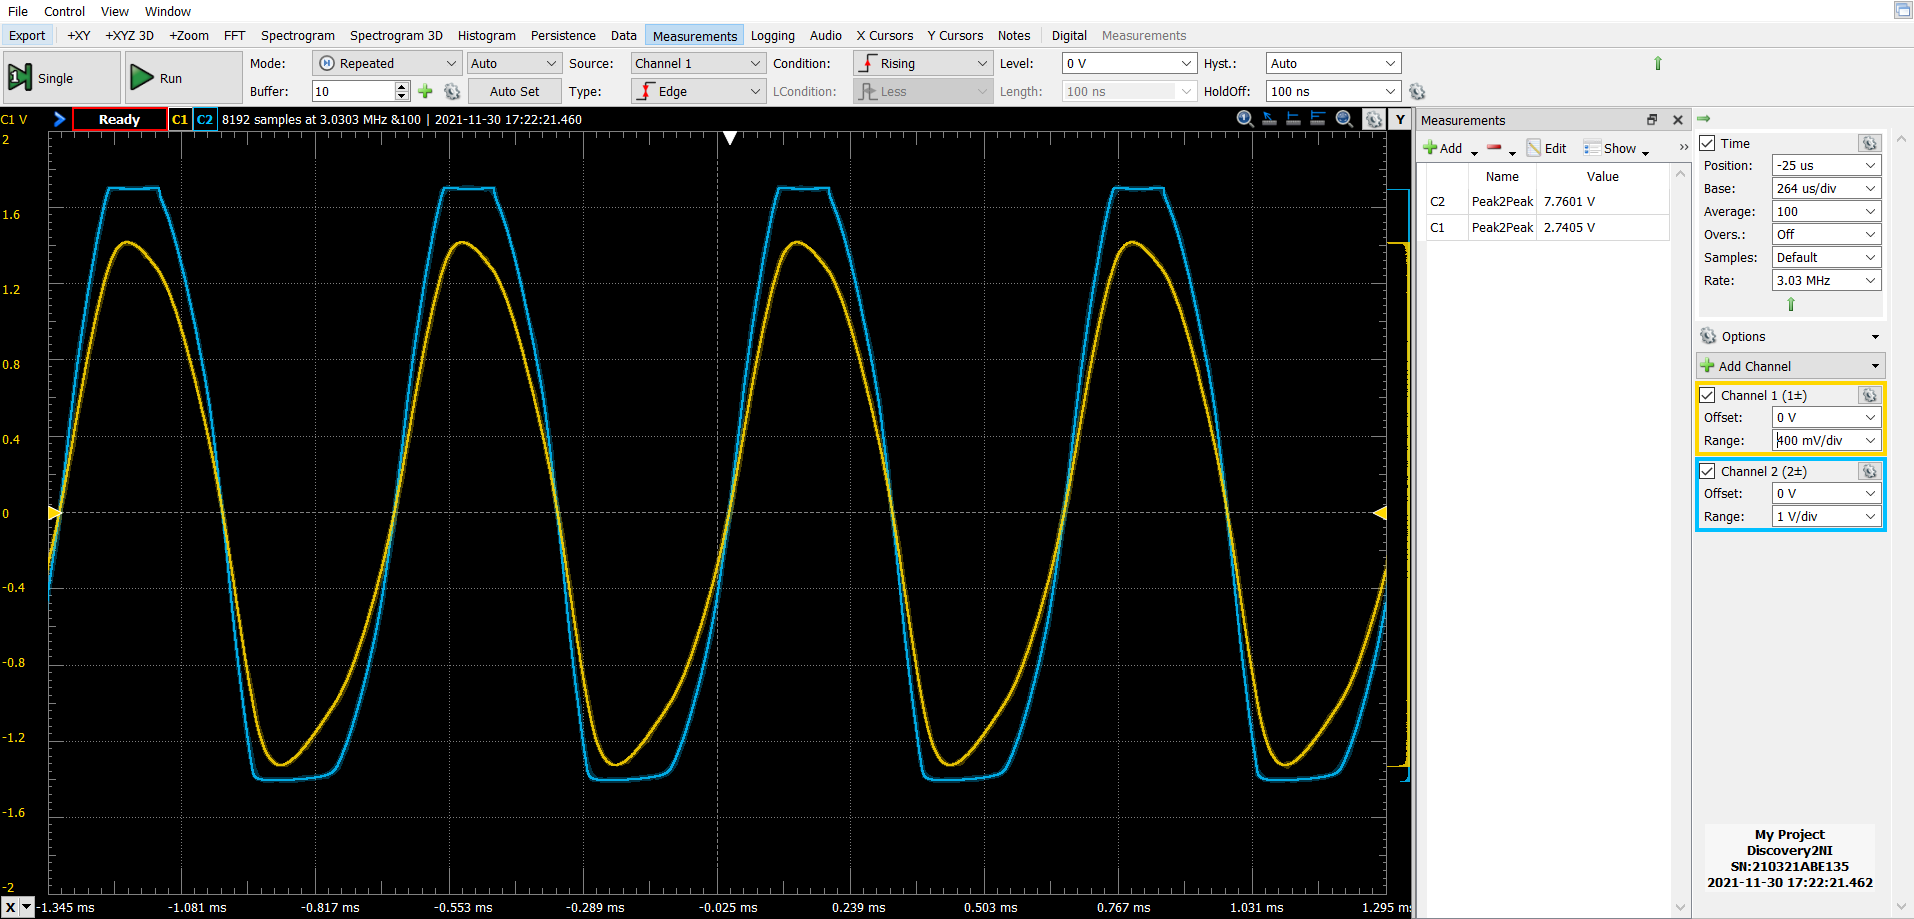
\includegraphics[scale=0.4]{4.60}
    \caption{situazione in cui il guadagno ad anello chiuso diverge; $R_{p2} =59.9 \pm 0.6 \si{\ohm}$, il segnale diverge fino alla saturazione, poi si stabilizza perchè incontra il suo massimo.
    \label{fig: Draft1}}
\end{figure}
Quando invece $R_{p2}$ è troppo basso il segnale tende invece a convergere: qualunque segnale, di qualunque ampiezza, si attenua fino a scomparire.
Un comportamento stabile (non saturato si intende) lo otteniamo in un intervallo limitato di valori per il potenziometro, per esempio quando $R_{p2} \approx 3 \si{k\ohm}$: in questa situazione il guadagno dell'anello amplificatore è sufficientemente alto per innescare l'oscillazione, ma non è nemmeno eccessivamente alto da permettere al segnale di divergere fino a saturazione; ciò che si ottiene in questo caso è che il valore del guadagno cambia nel tempo (grazie ai 2 diodi simmetrici messi in parallelo a $R_3$, come descritto prima) e oscilla vicino a 1. In questo modo otteniamo un'oscillazione sinusoidale stabile.
\begin{figure}[H]
    \centering
	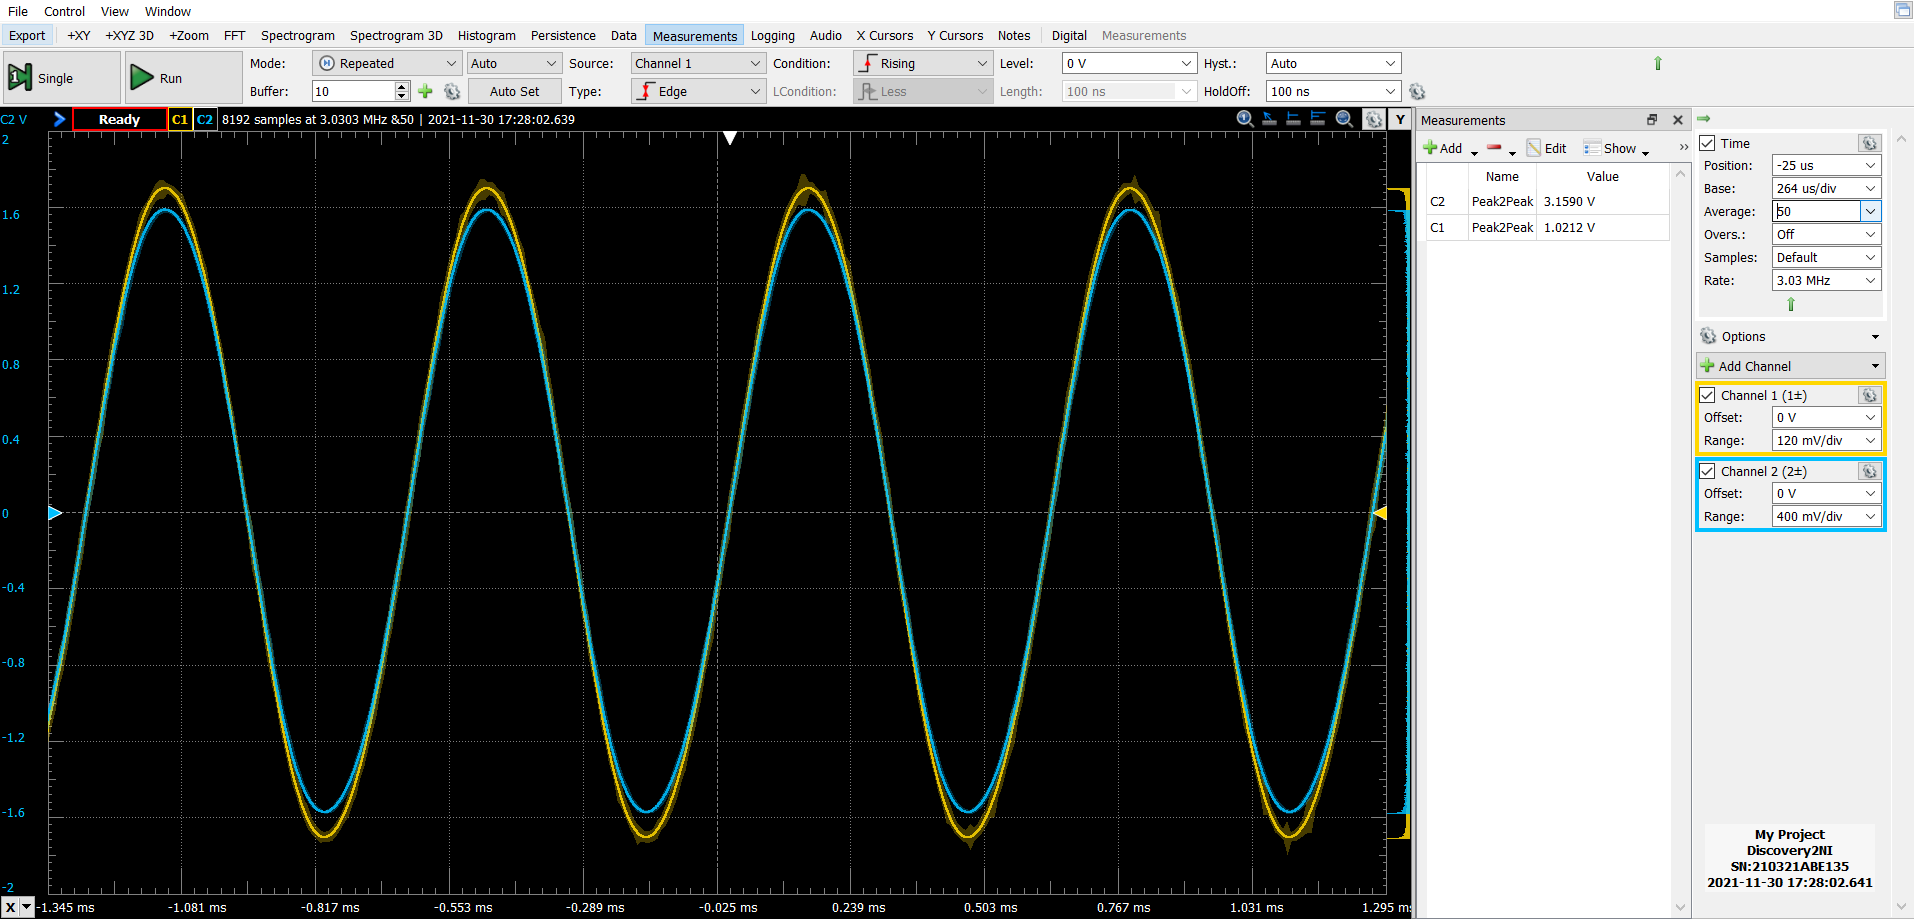
\includegraphics[scale=0.4]{4.2360}
    \caption{situazione in cui il guadagno ad anello chiuso risulta confinata in un intorno di 1; $R_{p1} =2.36 \pm 0.03 \si{k\ohm}$. Il segnale è stabile.
    \label{fig: Draft1}}
\end{figure}
Utilizzando i cursori si è misurata la frequenza dell'oscillazione:
\[
f=1.57 \pm 0.01 \si{kHz}
\]
la quale non sembra essere influenzata molto dal valore del potenziometro, infatti si è utilizzata la funzione measurements di waveforms per vederne l'andamento, stando attenti a non finire nella regione di saturazione del segnale: abbiamo identificato quindi un massimo e minimo di frequenza, che si aggirano intorno a $f= 1578 Hz$ e $f= 1568 Hz$ rispettivamente. L'ampiezza al contrario risulta cambiare di molto a seconda delle resistenze in gioco: chiaramente l'Ampiezza massima corrisponderà circa al valore di saturazione più vicino allo 0 (nel nostro caso risulta essere la tensione di saturazione negativa, pari a $V_{OL}=-3.43 \pm 0.04 V$), l'ampiezza minima invece è l'ampiezza misurata al valore di soglia del potenziometro, a cui avviene l'innesco, la quale misura $858 \pm 9 \si{m\V}$. Quest'ultima, come tutte le altre misure effettuate sul valore di soglia per cui avviene l'innesco, sono molto approssimative, poiché il potenziometro non è facilmente controllabile.
\subsection{Innesco dell'oscillazione}
Cortocircuitando un diodo e rilasciarlo successivamente ci dà l'opportunità di visualizzare l'innesco dell'oscillazione. Ci aspettiamo che per un valore più alto di $R_{p2}$ l'oscillazione impieghi meno tempo per arrivare alla stabilità, perché maggiore è il guadagno dell'anello amplificatore, maggiore sarà la velocità a cui il circuito raggiunge il regime di funzionamento stabile (non nullo).
\begin{figure}[H]
    \centering
	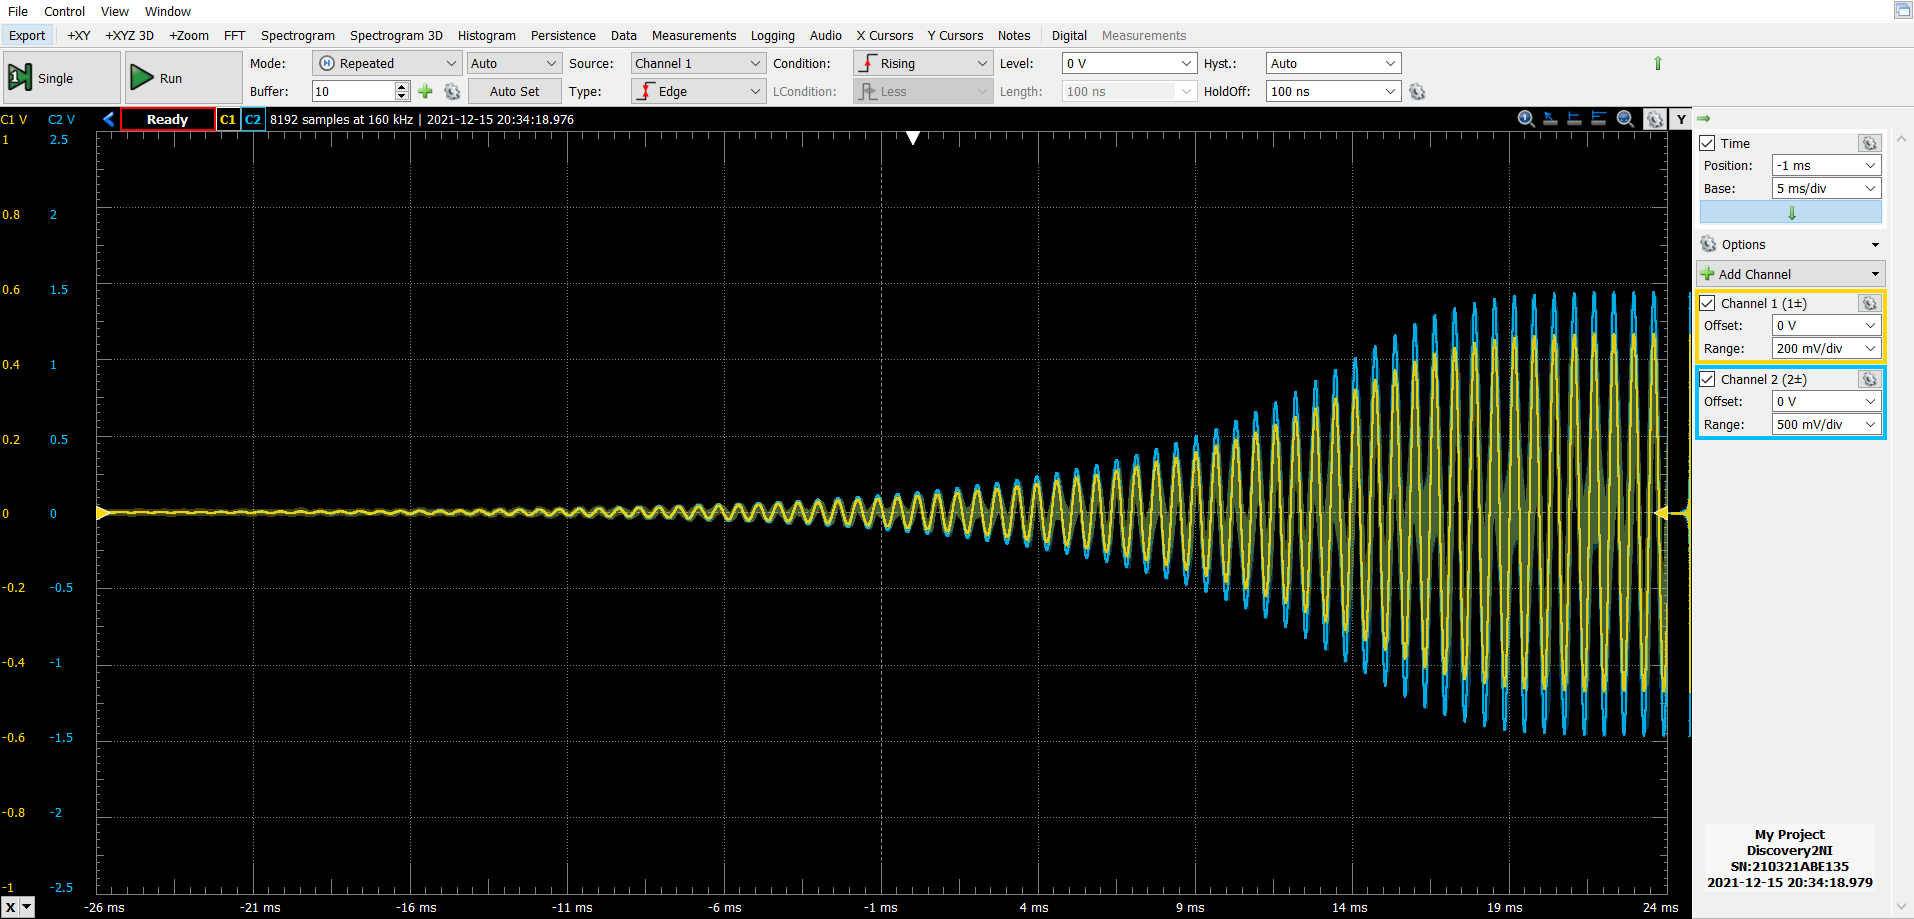
\includegraphics[scale=0.4]{5.7.26}
    \caption{innesco dell'oscillazione con $R_{p2}=7.26 \pm 0.06 \si{k\ohm}$
    \label{fig: Draft1}}
\end{figure}
\begin{figure}[H]
    \centering
	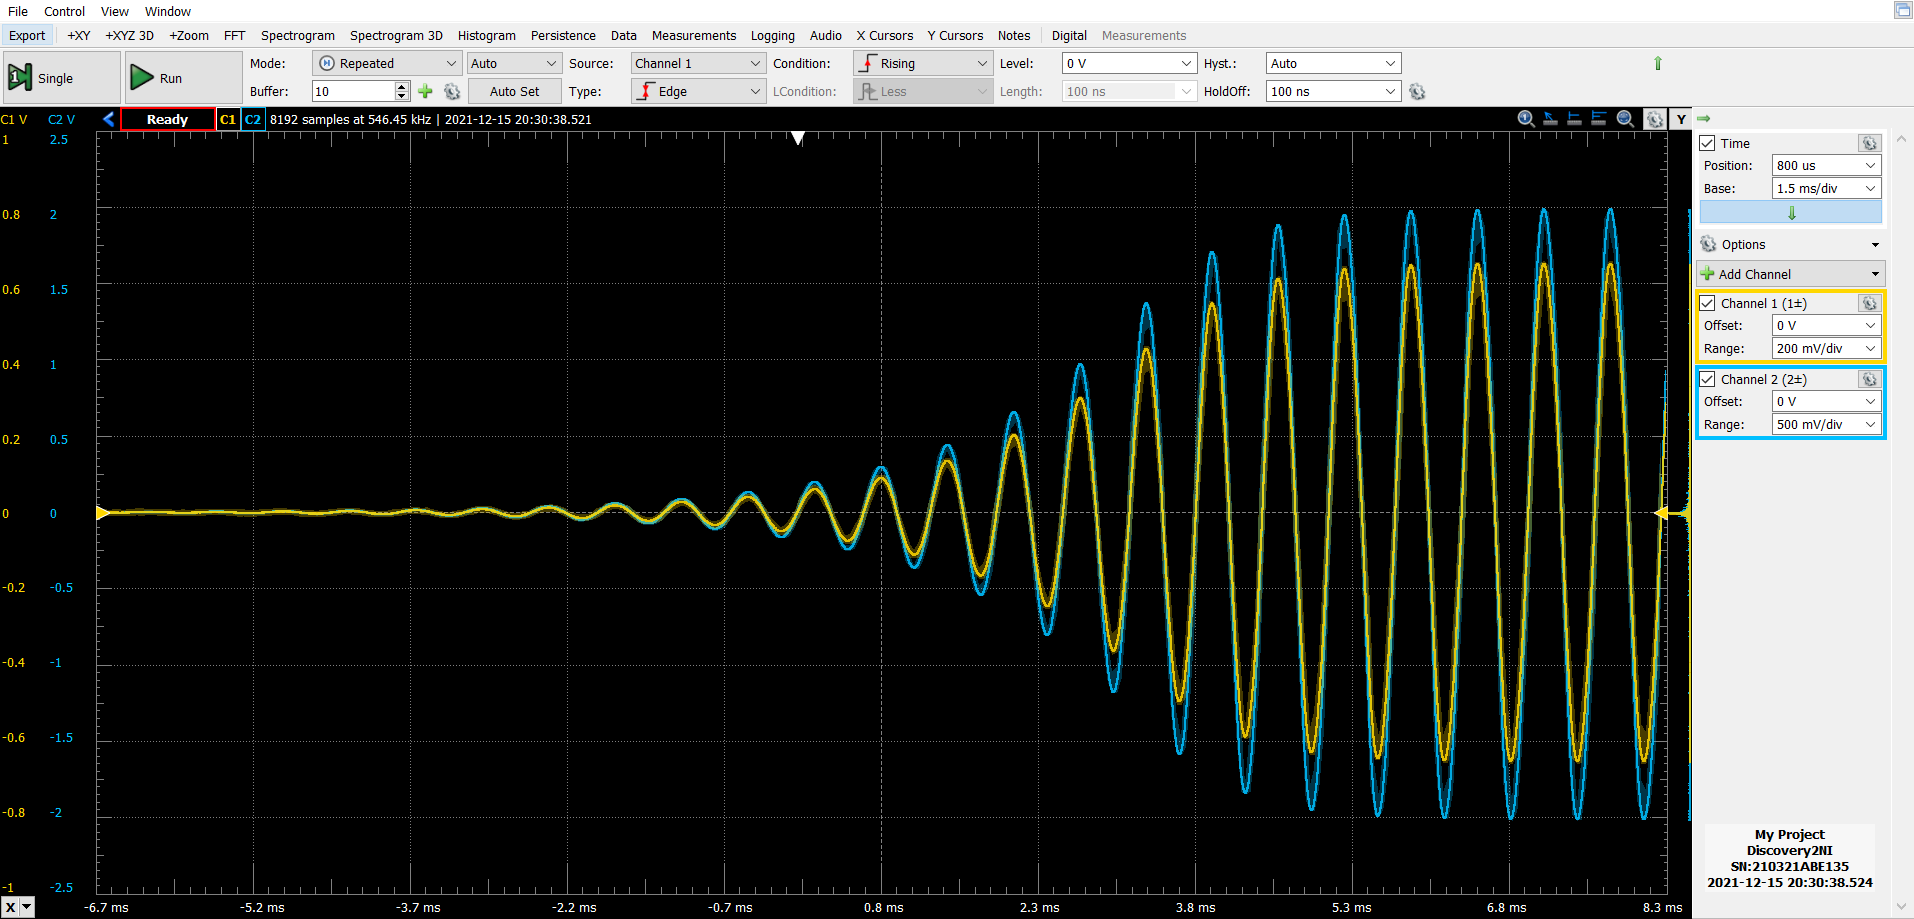
\includegraphics[scale=0.4]{5.7.63}
    \caption{innesco dell'oscillazione con $R_{p2}=7.63 \pm 0.06 \si{k\ohm}$
    \label{fig: Draft1}}
\end{figure}
Infatti mentre nel primo caso, con $R_{p2}=7.26 \pm 0.06 \si{k\ohm}$, il circuito impiega qualche decina di millisecondi per arrivare a regime, nel secondo caso, con $R_{p2}=7.63 \pm 0.06 \si{k\ohm}$, impiega solamente qualche millisecondo.
\subsection{Diodi}
Senza l'ausilio dei diodi non è possibile trovare una posizione del potenziometro per cui il circuito sia stabile (né segnale nullo, né in saturazione), infatti le uniche alternative sono o la saturazione del segnale, nel caso in cui con $R_{p2}$ sia troppo grosso, o la completa attenuazione del segnale, nel caso contrario.
\begin{figure}[H]
    \centering
	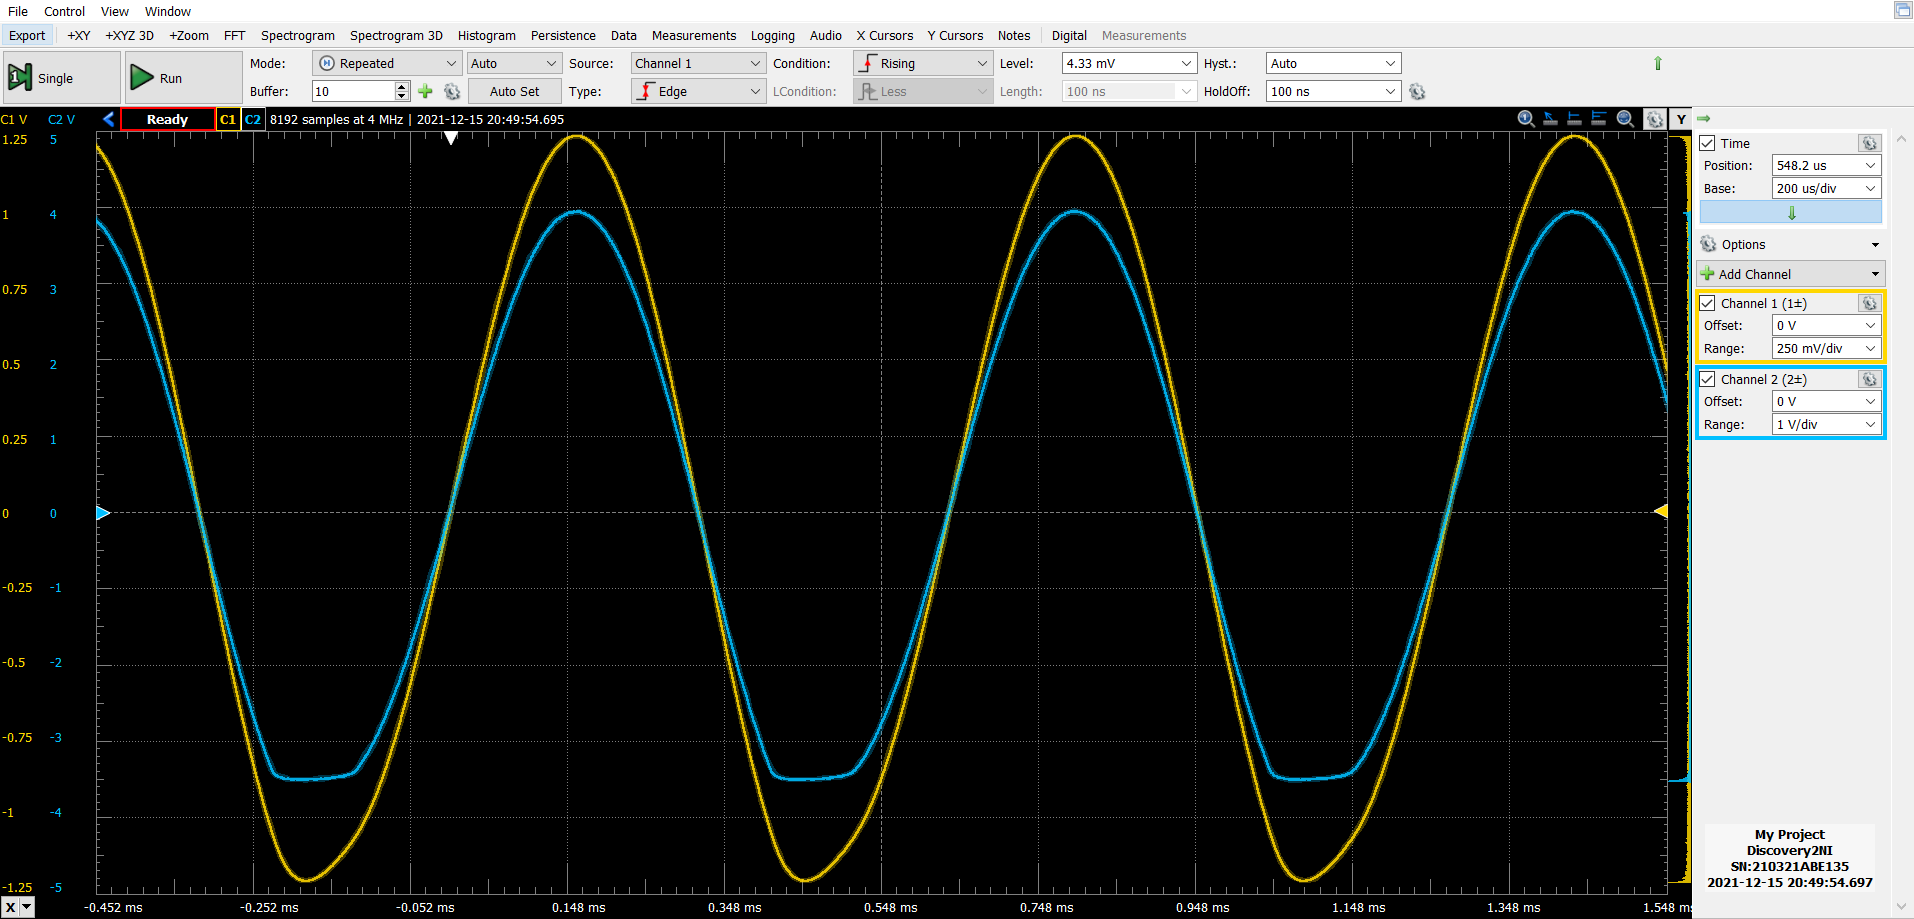
\includegraphics[scale=0.4]{senzadiodi}
    \caption{comportamento del circuito in assenza dei diodi: si nota come $R_{p2}$ sia troppo elevata, di conseguenza il segnale è entrato nella zona di saturazione, per questo la parte inferiore dell'onda in uscita risulta essere tagliata alla tensione di saturazione negativa dell'opAmp.
    \label{fig: Draft1}}
\end{figure}
La funzione dei diodi infatti è quella di variare dinamicamente il guadagno dell'anello: nel caso in cui il guadagno sia molto alto, per esempio all'innesco, la tensione ai capi dei diodi (e di $R_3$) aumenta; questo provoca la polarizzazione diretta dei diodi, la cui resistenza diminuisce, il che porta la resistenza costituita da $D_1$,$D_2$ e $R_3$ a diminuire, abbassando il guadagno dell'anello. Abbassando il guadagno però la resistenza dei diodi aumenta nuovamente, e di conseguenza quella del nodo, il che provoca un altro aumento del guadagno dell'anello; il ruolo è quindi quella di bilanciare il guadagno dell'amplificatore.
Nel caso in cui una perturbazione provochi un cambiamento nel segnale, i diodi cercheranno autonomamente di riportare il circuito in uno stato stabile: per esempio se il segnale aumentasse la resistenza dei diodi diminuirebbe, provocando un'attenuazione nel guadagno, in modo che il segnale torni allo stato di stabilità.
Senza questi sarebbe empiricamente impossibile trovare una situazione in cui il guadagno totale $L(j\omega) $ sia pari a 1, con l'uniche possibilità che il circuito o diverga fino a saturare, o si attenui fino al segnale nullo.
\subsection{Misura del guadagno $A_v$}
Lasciando il potenziometro fisso al valore di soglia per cui il circuito innesca l'oscillazione, pari a $R_{p2}=7.37 \pm 0.06 \si{k\ohm}$, si è disconnesso l'entrata non invertente dell'opAmp dal punto A, e si è collegata ad un generatore di segnali. Si è quindi inviato un segnale sinusoidale a frequenza $1.58 kHz$ e ampiezza $201 \pm 2 \si{m\V}$. Abbiamo quindi misurato $V_{out}=620 \pm 5 \si{m\V}$ e un guadagno pari a
\[
A=3.10 \pm 0.04
\]
Nonostante sia lontano 2 barre di errore dal valore aspettato, c'è da dire che il potenziometro non è uno strumento di precisione, perché anche al minimo tocco si può spostare la resistenza $R_{p2}$ o $R_{p1}$ che sia anche di 80 ohm, il che non ci permette di avvicinarci a sufficienza al valore di soglia; fatta questa premessa posso quindi dire che il valore misurato è compatibile con le aspettative.
%=======================
\section*{Dichiarazione}
I firmatari di questa relazione dichiarano che il contenuto della relazione \`e
originale, con misure effettuate dai membri del gruppo, e che tutti i firmatari
hanno contribuito alla elaborazione della relazione stessa.

\end{document}
